\newpage

\chapter*{Appendix}\label{sec:appendix}
\addcontentsline{toc}{chapter}{Appendix}
\markboth{Appendix}{Appendix}

%%% l2 norm results

\begin{figure}[ht] % "[t!]" placement specifier just for this example
	\centering
\includegraphics[width=.7\linewidth]{\detokenize{./images/compact/fcnn_l2_17.60}}
\caption{FCNN Example Images ($l_2$-Norm) \\ with an input PSNR of 17.60} \label{fig:e}

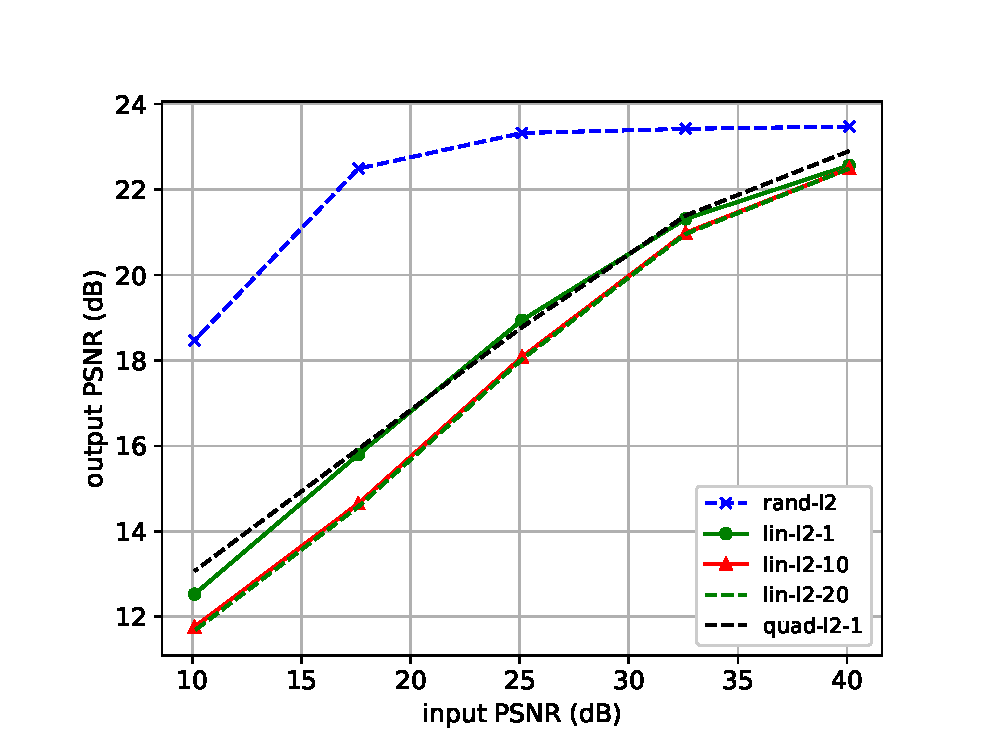
\includegraphics[width=.7\linewidth]{\detokenize{./images/figures/fcnn_fig_mnist_l2}}
\caption{FCNN PSNR Figure ($l_2$-Norm)} \label{fig:f}
\end{figure}


\begin{figure}[ht]
	\centering
\includegraphics[width=.7\linewidth]{\detokenize{./images/compact/fcnn2_l2_17.60}}
\caption{FCNN2 Example Images ($l_2$-Norm) \\ with an input PSNR of 17.60} \label{fig:e}

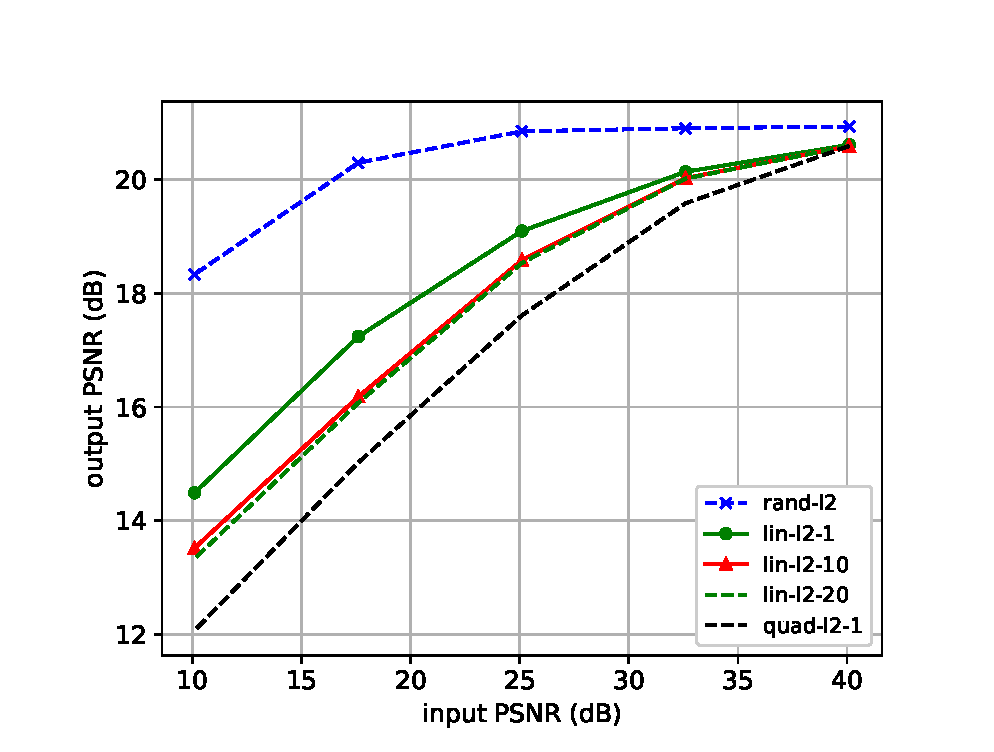
\includegraphics[width=.7\linewidth]{\detokenize{./images/figures/fcnn2_fig_mnist_l2}}
\caption{FCNN2 PSNR Figure ($l_2$-Norm)} \label{fig:f}
\end{figure}


\begin{figure}[ht]
	\centering
\includegraphics[width=.7\linewidth]{\detokenize{./images/compact/fcnn3_l2_14.87}}
\caption{FCNN3 Example Images ($l_2$-Norm) \\ with an input PSNR of 14.87} \label{fig:e}

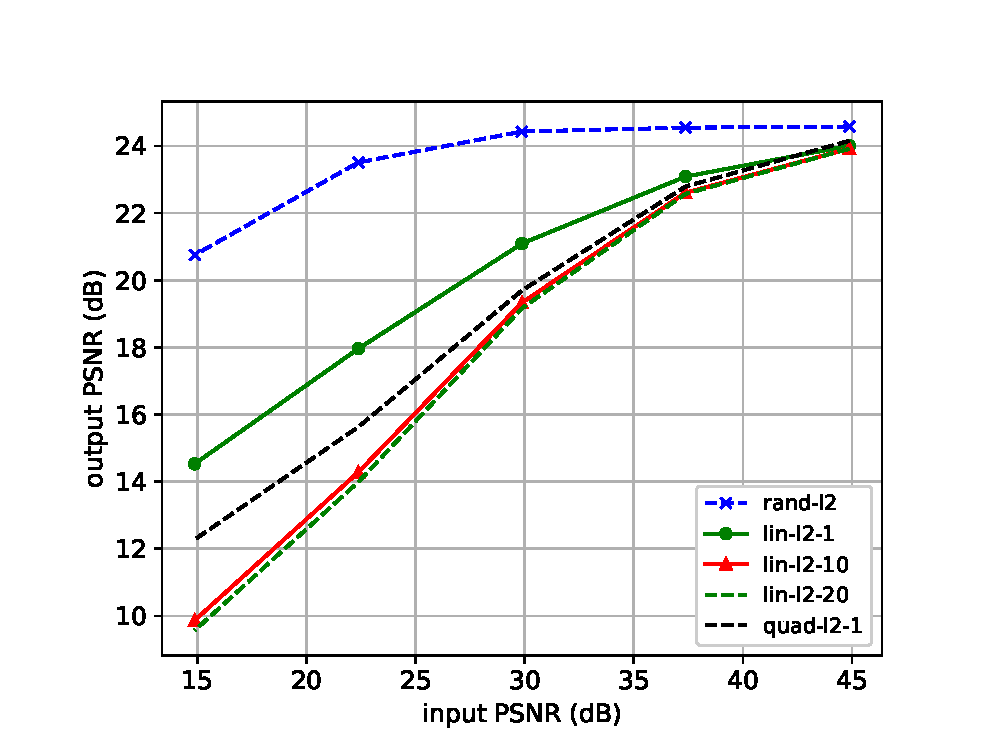
\includegraphics[width=.7\linewidth]{\detokenize{./images/figures/fcnn3_fig_cifar_l2}}
\caption{FCNN3 PSNR Figure ($l_2$-Norm)} \label{fig:fcnn3_l2}
\end{figure}


\begin{figure}[ht]
	\centering
\includegraphics[width=.7\linewidth]{\detokenize{./images/compact/aen_stl10_l2_31.92}}
\caption{AEN\_STL10 Example Images ($l_2$-Norm) \\ with an input PSNR of 31.92} \label{fig:e}

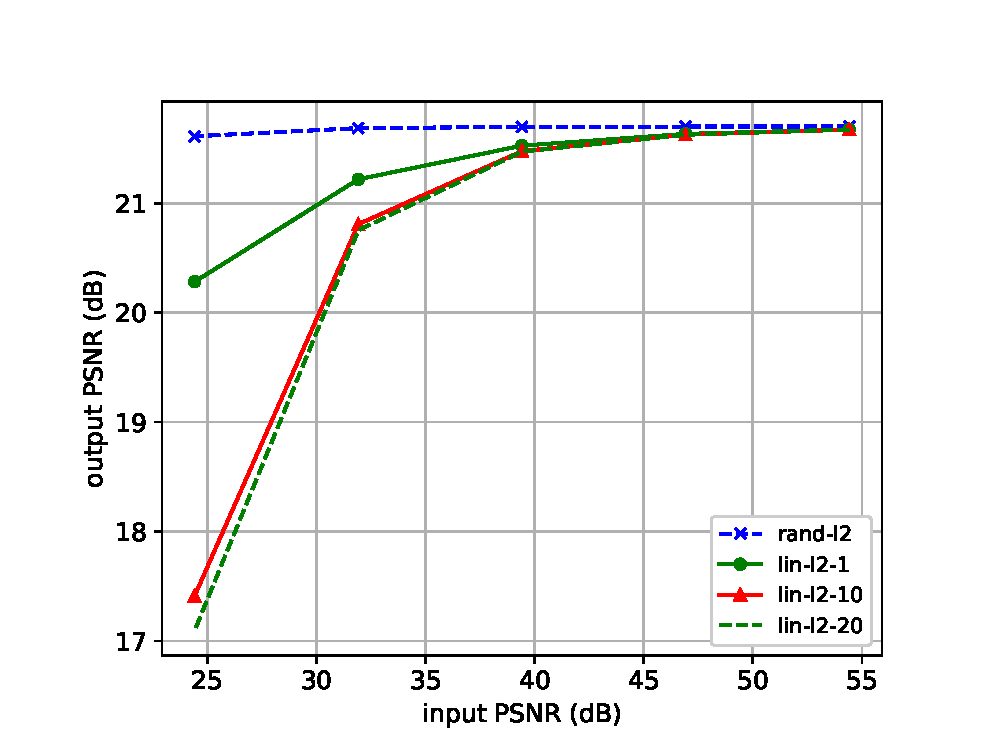
\includegraphics[width=.7\linewidth]{\detokenize{./images/figures/aen_stl10_fig_stl10_l2}}
\caption{AEN\_STL10 PSNR Figure ($l_2$-Norm)} \label{fig:f}
\end{figure}


\begin{figure}[ht]
	\centering
\includegraphics[width=.7\linewidth]{\detokenize{./images/compact/koala_l2_31.92}}
\caption{KOALA Example Images ($l_2$-Norm) \\ with an input PSNR of 31.92} \label{fig:e}

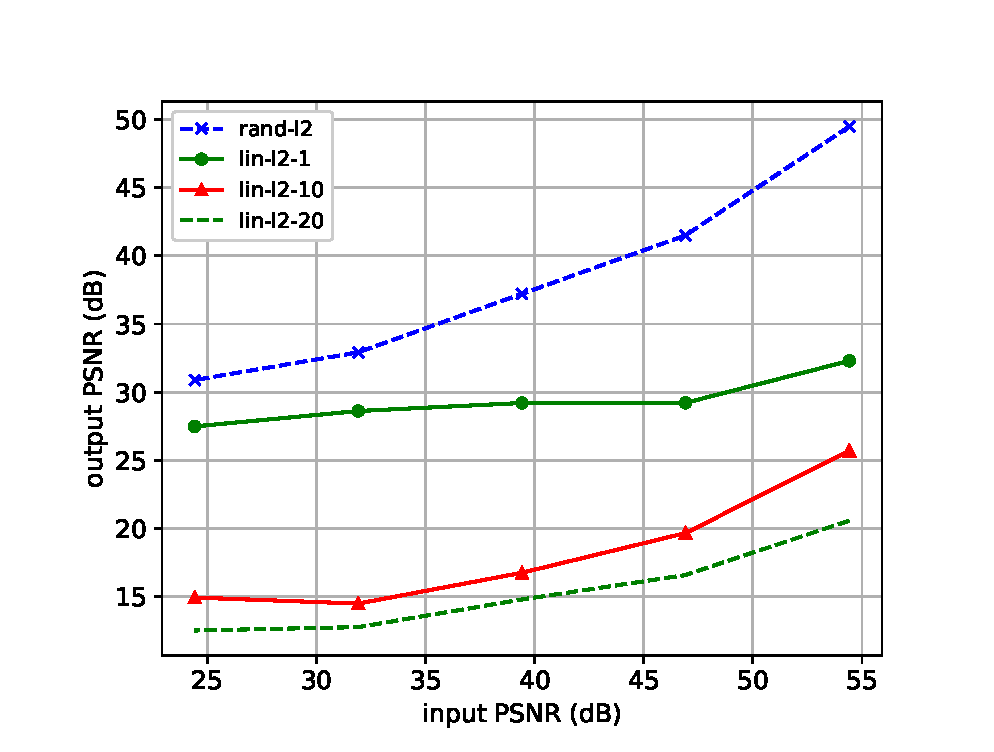
\includegraphics[width=.7\linewidth]{\detokenize{./images/figures/koala_fig_stl10_l2}}
\caption{KOALA PSNR Figure ($l_2$-Norm)} \label{fig:f}
\end{figure}


\begin{figure}[ht]
	\centering
\includegraphics[width=.7\linewidth]{\detokenize{./images/compact/c_dcscn_l2_26.02}}
\caption{C\_DCSCN Example Images ($l_2$-Norm) \\ with an input PSNR of 26.02} \label{fig:e}

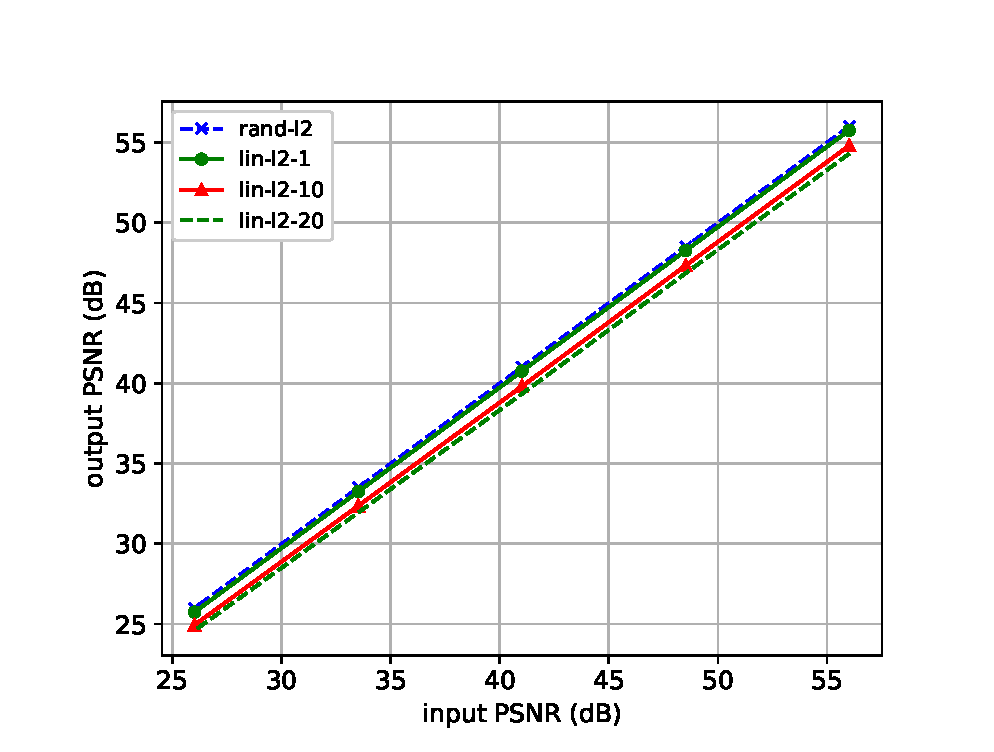
\includegraphics[width=.7\linewidth]{\detokenize{./images/figures/c_dcscn_fig_set14_l2}}
\caption{C\_DCSCN PSNR Figure ($l_2$-Norm)} \label{fig:f}
\end{figure}

%%% linf norm results

\begin{figure}[ht]
	\centering
\includegraphics[width=.7\linewidth]{\detokenize{./images/compact/fcnn_linf_17.50}}
\caption{FCNN Example Images ($l_\infty$-Norm) \\ with an input PSNR of 17.50} \label{fig:e}

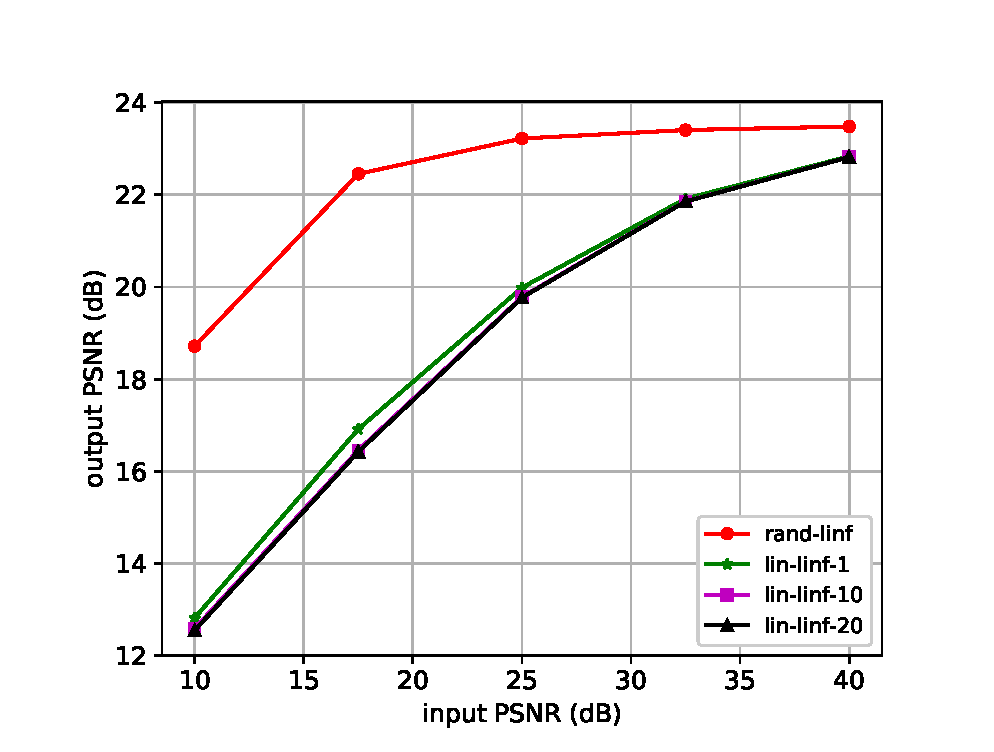
\includegraphics[width=.7\linewidth]{\detokenize{./images/figures/fcnn_fig_mnist_linf}}
\caption{FCNN PSNR Figure ($l_\infty$-Norm)} \label{fig:f}
\end{figure}

\begin{figure}[ht]
	\centering
\includegraphics[width=.7\linewidth]{\detokenize{./images/compact/fcnn2_linf_17.50}}
\caption{FCNN2 Example Images ($l_\infty$-Norm) \\ with an input PSNR of 17.50} \label{fig:e}

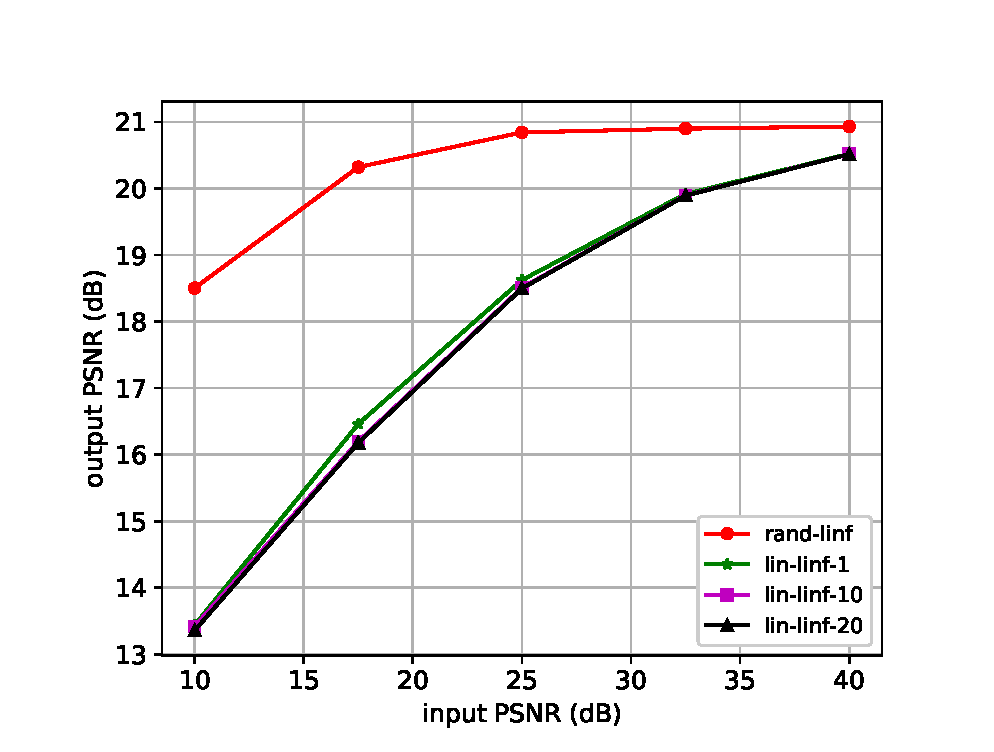
\includegraphics[width=.7\linewidth]{\detokenize{./images/figures/fcnn2_fig_mnist_linf}}
\caption{FCNN2 PSNR Figure ($l_\infty$-Norm)} \label{fig:f}
\end{figure}

\begin{figure}[ht]
	\centering
\includegraphics[width=.7\linewidth]{\detokenize{./images/compact/fcnn3_linf_17.50}}
\caption{FCNN3 Example Images ($l_\infty$-Norm) \\ with an input PSNR of 17.50} \label{fig:e}

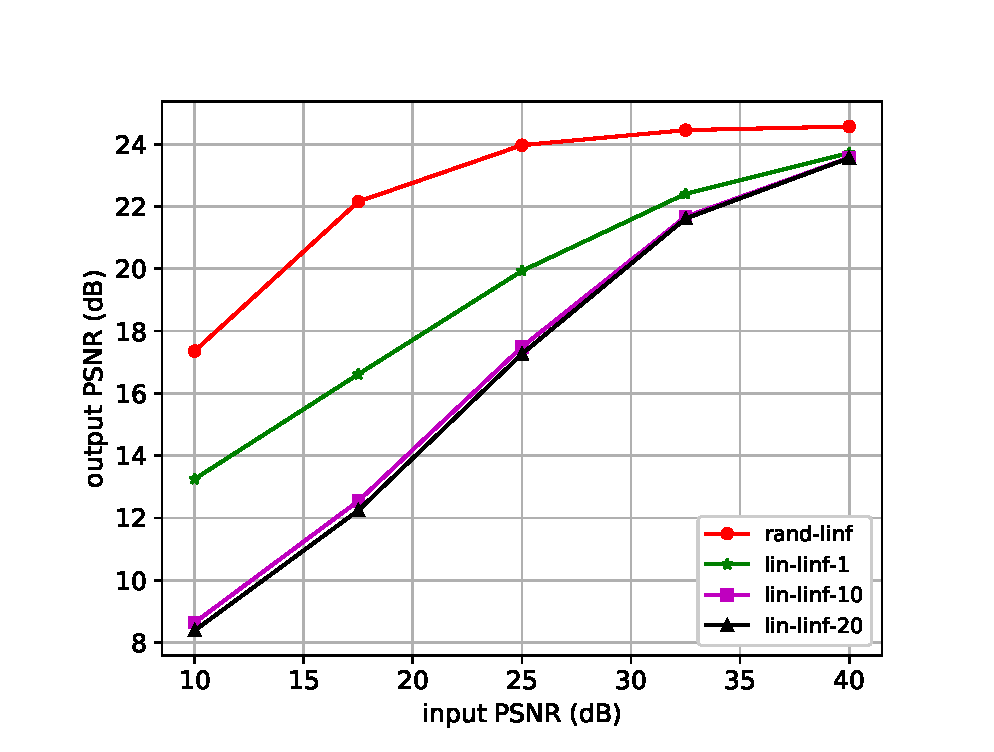
\includegraphics[width=.7\linewidth]{\detokenize{./images/figures/fcnn3_fig_cifar_linf}}
\caption{FCNN3 PSNR Figure ($l_\infty$-Norm)} \label{fig:f}
\end{figure}

\begin{figure}[ht]
	\centering
\includegraphics[width=.7\linewidth]{\detokenize{./images/compact/aen_stl10_linf_17.50}}
\caption{AEN\_STL10 Example Images ($l_\infty$-Norm) \\ with an input PSNR of 17.50} \label{fig:e}

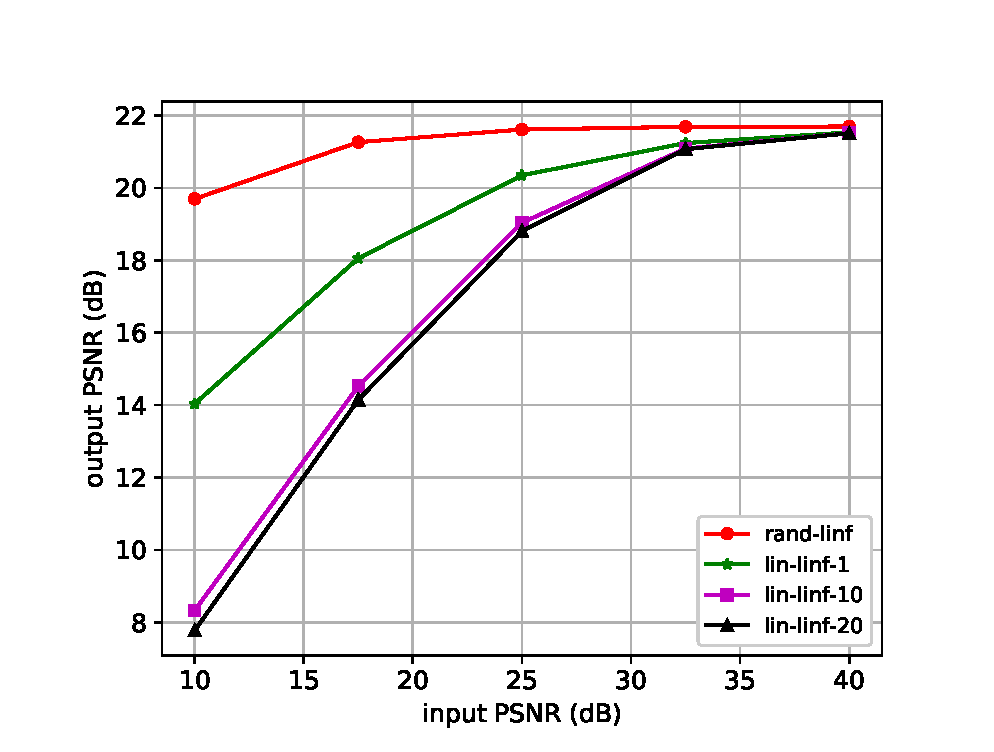
\includegraphics[width=.7\linewidth]{\detokenize{./images/figures/aen_stl10_fig_stl10_linf}}
\caption{AEN\_STL10 PSNR Figure ($l_\infty$-Norm)} \label{fig:f}
\end{figure}

\begin{figure}[ht]
	\centering
\includegraphics[width=.7\linewidth]{\detokenize{./images/compact/koala_linf_17.50}}
\caption{KOALA Example Images ($l_\infty$-Norm) \\ with an input PSNR of 17.50} \label{fig:e}

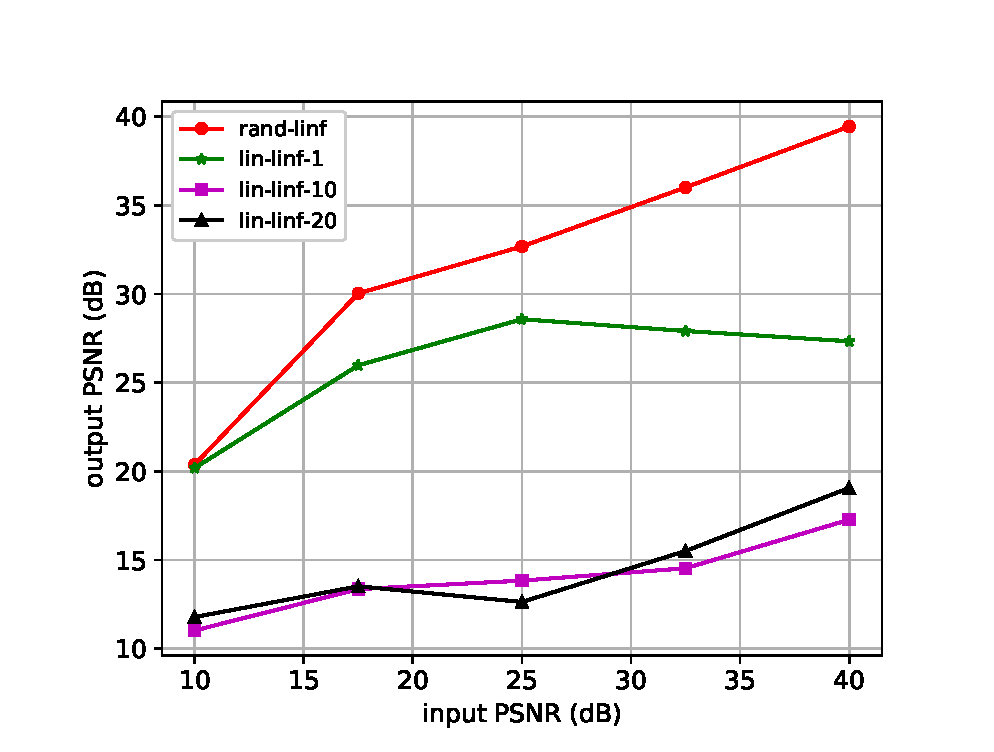
\includegraphics[width=.7\linewidth]{\detokenize{./images/figures/koala_fig_stl10_linf}}
\caption{KOALA PSNR Figure ($l_\infty$-Norm)} \label{fig:f}
\end{figure}

\begin{figure}[ht]
	\centering
\includegraphics[width=.7\linewidth]{\detokenize{./images/compact/c_dcscn_linf_17.50}}
\caption{C\_DCSCN Example Images ($l_\infty$-Norm) \\ with an input PSNR of 17.50} \label{fig:e}

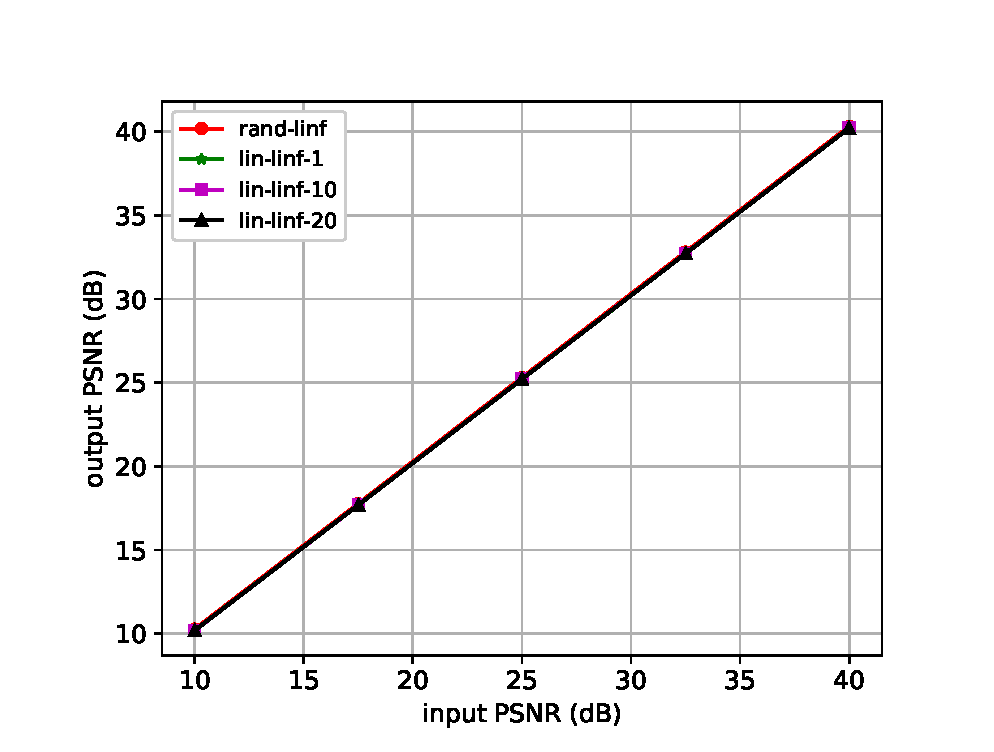
\includegraphics[width=.7\linewidth]{\detokenize{./images/figures/c_dcscn_fig_set14_linf}}
\caption{C\_DCSCN PSNR Figure ($l_\infty$-Norm)} \label{fig:f}
\end{figure}

%% pixel attack

\begin{figure}[ht]
	\centering
\includegraphics[width=.7\linewidth]{\detokenize{./images/compact/fcnn_pixel_0.20}}
\caption{FCNN Example Images \\ with an input $\epsilon \;$ of 0.20} \label{fig:e}

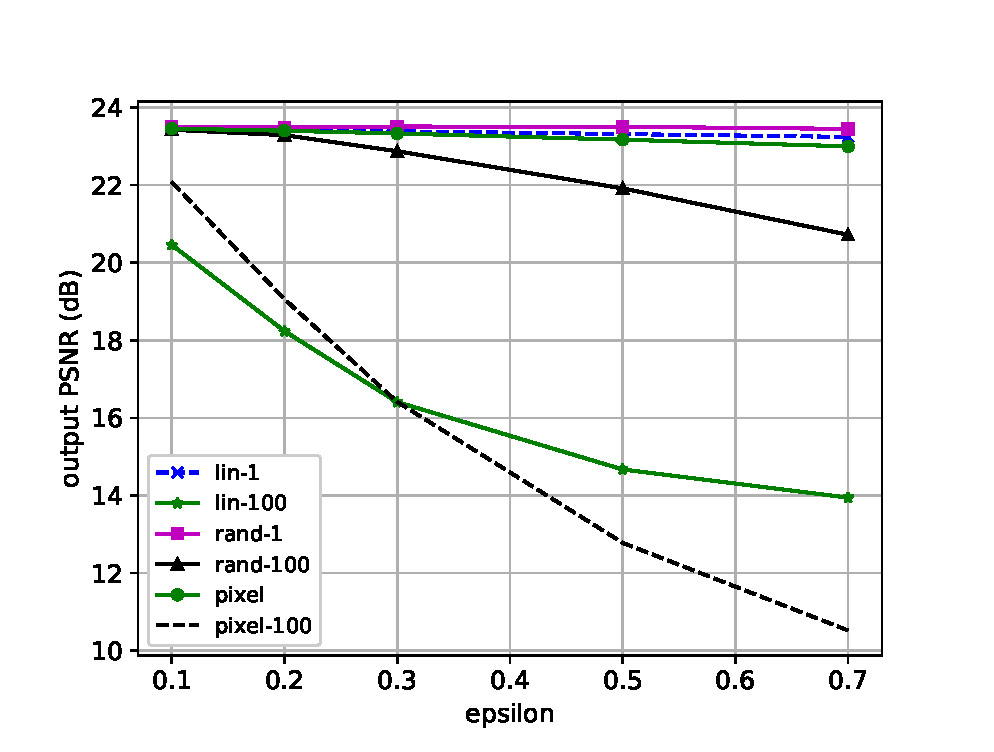
\includegraphics[width=.7\linewidth]{\detokenize{./images/figures/fcnn_fig_mnist_pixel}}
\caption{FCNN PSNR Figure (Single Subset Attack)} \label{fig:f}
\end{figure}

\begin{figure}[ht]
	\centering
\includegraphics[width=.7\linewidth]{\detokenize{./images/compact/fcnn2_pixel_0.20}}
\caption{FCNN2 Example Images \\ with an input $\epsilon \;$ of 0.20} \label{fig:e}

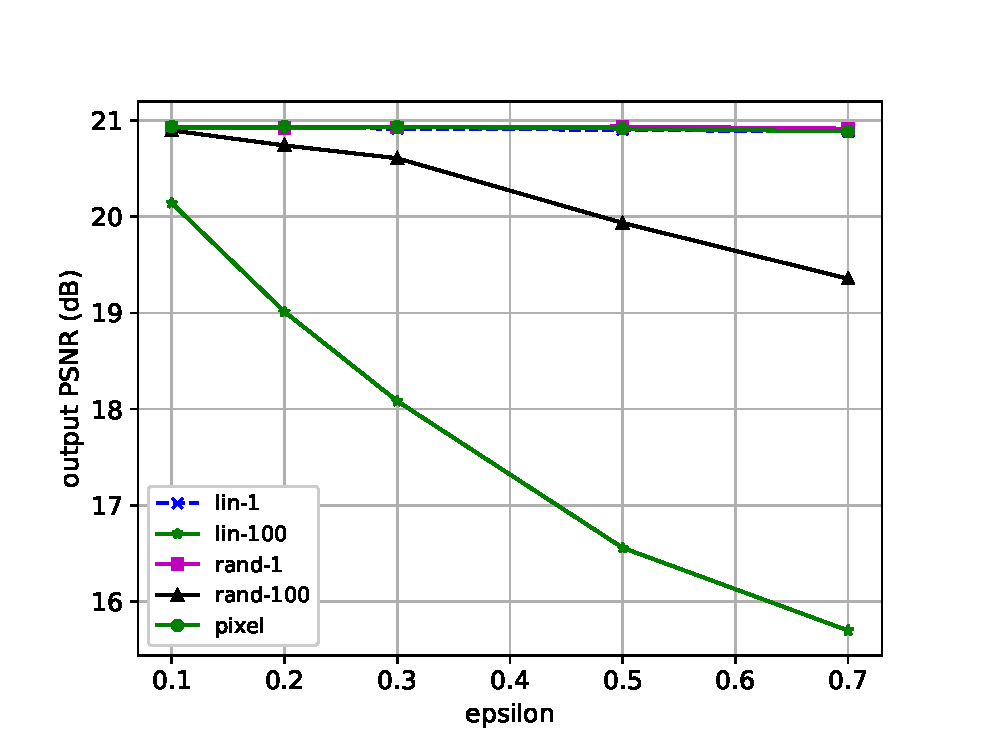
\includegraphics[width=.7\linewidth]{\detokenize{./images/figures/fcnn2_fig_mnist_pixel}}
\caption{FCNN2 PSNR Figure (Single Subset Attack)} \label{fig:f}
\end{figure}

\begin{figure}[ht]
	\centering
\includegraphics[width=.7\linewidth]{\detokenize{./images/compact/fcnn3_pixel_0.20}}
\caption{FCNN3 Example Images \\ with an input $\epsilon \;$ of 0.20} \label{fig:e}

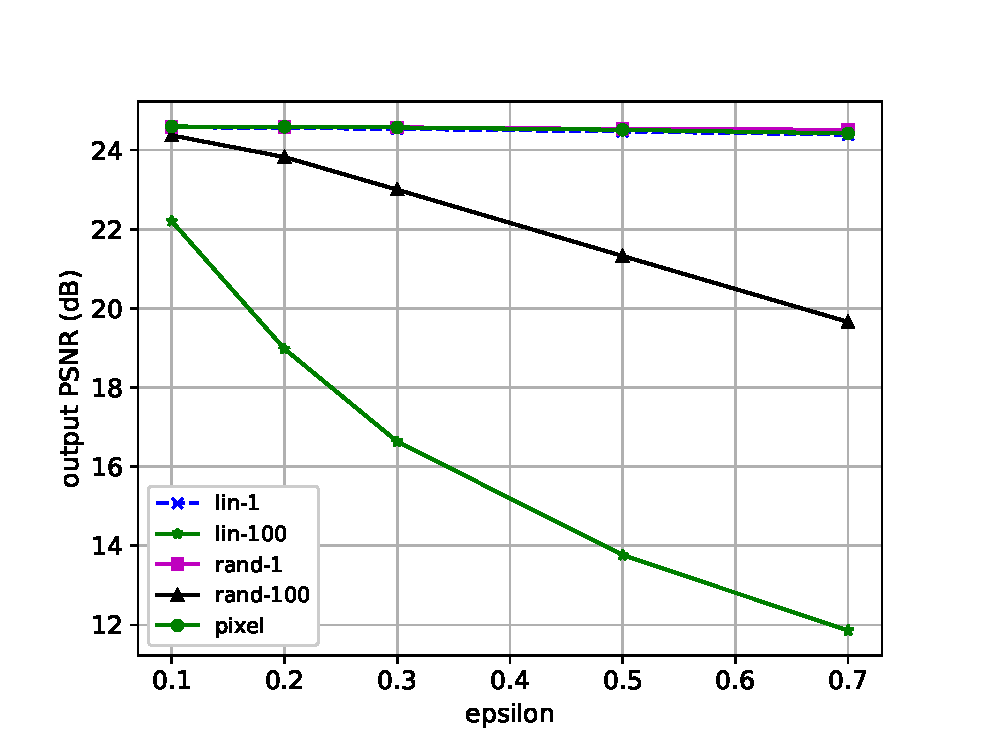
\includegraphics[width=.7\linewidth]{\detokenize{./images/figures/fcnn3_fig_cifar_pixel}}
\caption{FCNN3 PSNR Figure (Single Subset Attack)} \label{fig:f}
\end{figure}

\begin{figure}[ht]
	\centering
\includegraphics[width=.7\linewidth]{\detokenize{./images/compact/aen_stl10_pixel_0.20}}
\caption{AEN\_STL10 Example Images \\ with an input $\epsilon \;$ of 0.20} \label{fig:e}

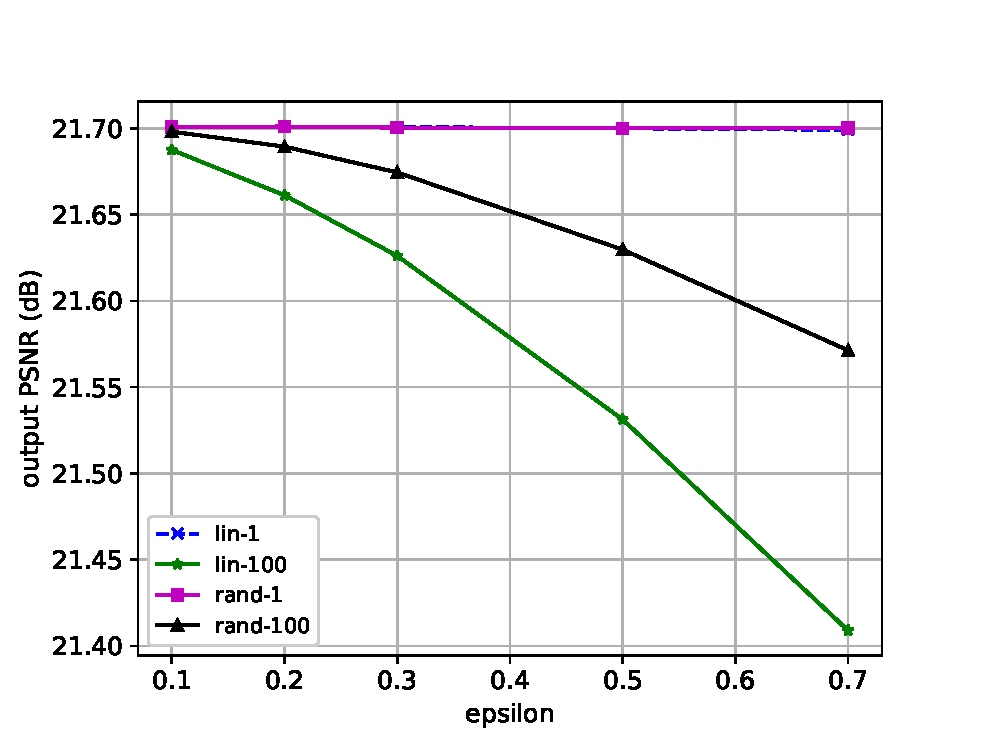
\includegraphics[width=.7\linewidth]{\detokenize{./images/figures/aen_stl10_fig_stl10_pixel}}
\caption{AEN\_STL10 PSNR Figure (Single Subset Attack)} \label{fig:f}
\end{figure}

\begin{figure}[ht]
	\centering
\includegraphics[width=.7\linewidth]{\detokenize{./images/compact/koala_pixel_0.20}}
\caption{KOALA Example Images \\ with an input $\epsilon \;$ of 0.20} \label{fig:e}

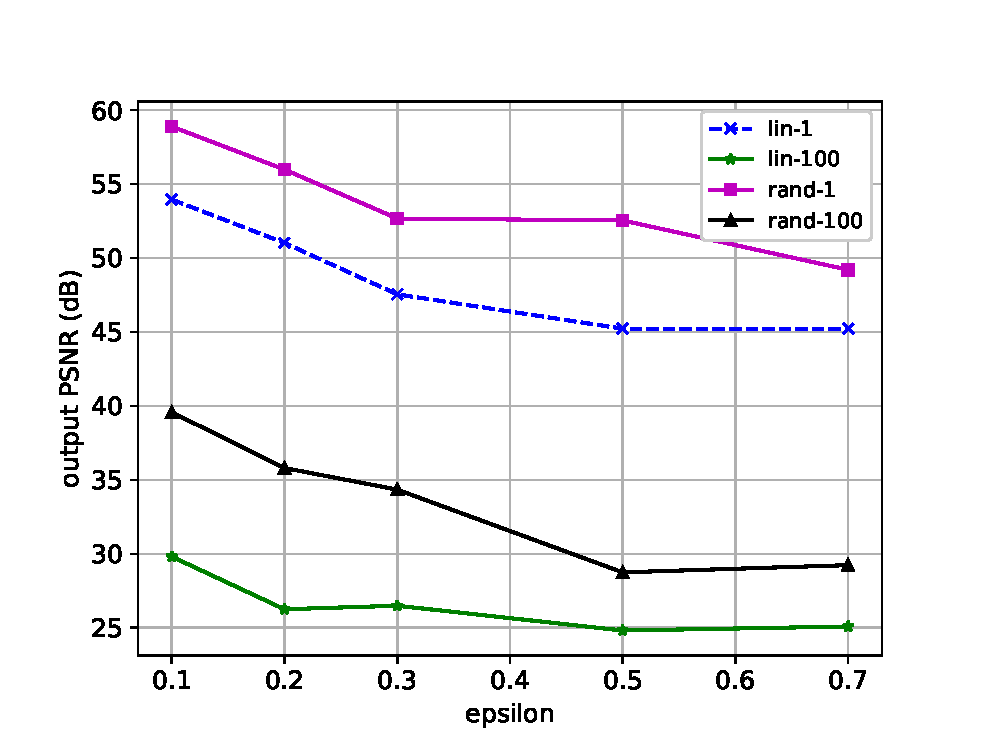
\includegraphics[width=.7\linewidth]{\detokenize{./images/figures/koala_fig_stl10_pixel}}
\caption{KOALA PSNR Figure (Single Subset Attack)} \label{fig:f}
\end{figure}
